\section{Auswertung}
\label{sec:Auswertung}

\begin{table}[H]
  \centering
  \caption{Alle aufgenommenen Größen in Abhängigkeit der Zeit in Ablesereihenfolge.}
  \label{tab:messwerte}
  \begin{tblr}{
    colspec={S[table-format=2.2] S[table-format=2.2] S[table-format=2.2] S[table-format=2.2] S[table-format=2.2] 
    S[table-format=2.2]},
    row{1}={guard, mode=math},}
    \toprule
    t\mathbin{/}\unit{\minute} & A\mathbin{/}\unit{\watt} & p_{\symup{b}}\mathbin{/}\unit{\bar} & T_1\mathbin{/}°C &
    T_2\mathbin{/}°C & p_{\symup{a}}\mathbin{/}\unit{\bar} \\
    \midrule
    0   &    0    &   3.5   &   20.5  &   20.6  &   3.8   \\       
    1   &    110  &   5.0   &   21.4  &   20.5  &   3.0   \\
    2   &    115  &   5.0   &   22.8  &   19.1  &   3.3   \\
    3   &    120  &   5.5   &   24.2  &   17.8  &   3.4   \\
    4   &    120  &   6.0   &   25.9  &   16.4  &   3.5   \\
    5   &    120  &   6.0   &   27.6  &   15.0  &   3.4   \\
    6   &    120  &   6.5   &   28.9  &   14.2  &   3.2   \\
    7   &    120  &   7.0   &   30.4  &   13.2  &   3.0   \\
    8   &    120  &   7.0   &   31.6  &   12.2  &   3.0   \\
    9   &    125  &   7.0   &   33.0  &   11.2  &   2.9   \\
    10  &    125  &   7.5   &   34.2  &   10.3  &   2.7   \\
    11  &    125  &   8.0   &   35.4  &   9.2   &   2.7   \\
    12  &    125  &   8.0   &   36.5  &   8.4   &   2.6   \\
    13  &    125  &   8.0   &   37.6  &   7.6   &   2.4   \\
    14  &    125  &   8.5   &   38.6  &   6.7   &   2.4   \\
    15  &    115  &   9.0   &   39.6  &   5.8   &   2.2   \\
    16  &    115  &   9.0   &   40.5  &   5.0   &   2.2   \\
    17  &    115  &   9.0   &   41.4  &   4.3   &   2.1   \\
    18  &    115  &   9.5   &   42.3  &   3.6   &   2.0   \\
    19  &    115  &   9.5   &   43.1  &   2.9   &   2.0   \\
    20  &    115  &   10.0  &   43.9  &   2.2   &   1.9   \\
    21  &    115  &   10.0  &   44.6  &   1.6   &   1.9   \\ 
    22  &    115  &   10.0  &   45.4  &   1.0   &   1.8   \\ 
    23  &    110  &   10.5  &   46.0  &   0.4   &   1.8   \\
    24  &    110  &   10.5  &   46.6  &   -0.2  &   1.8   \\ 
    \bottomrule
  \end{tblr}
\end{table} 
Dabei hat die Leistung $A$ einen Ablesefehler von $\qty{5}{\watt}$, $p_{\symup{b}}$ einen von $\qty{0.5}{\bar}$, $T_1$ und $T_2$ einen von
$0.1°C$ und $p_{\symup{a}}$ einen Fehler von $\qty{0.1}{\bar}$.
\subsection{Temperaturverläufe}
In Abbildung \ref{fig:plot} werden die Temperaturverläufe von $T_1$ und $T_2$ dargestellt.
Hier wurde die Temperatur in Kelvin und die Zeit in Sekunden umgerechnet.
Für beide Verläufe wurde eine Ausgleichsfunktion als quadratisches Polynom gezeichnet.
Diese werden mit der Gleichung
\begin{equation*}
  f=a*t^2+b*t+c
\end{equation*}
beschrieben.
Dabei sind die Koeffizienten bei $T_1$
\begin{gather}
  a_{\symup{T}1}=\qty{-6.155(0.22)e-6}{\kelvin\per\second\squared}\\
  b_{\symup{T}1}=\qty{0.02742(0.00033)}{\kelvin\per\second}\\
  c_{\symup{T}1}=\qty{293(0.1)}{\kelvin}
  \label{eqn:fkt1}
\end{gather}
und bei $T_2$
\begin{gather}
  a_{\symup{T}2}=\qty{4.122(0.249)e-6}{\kelvin\per\second\squared}\\
  b_{\symup{T}2}=\qty{0.02078(0.00037)}{\kelvin\per\second}\\
  c_{\symup{T}2}=\qty{294.4(0.12)}{\kelvin}
  \label{eqn:fkt2}
\end{gather}
.

\begin{figure}[H]
  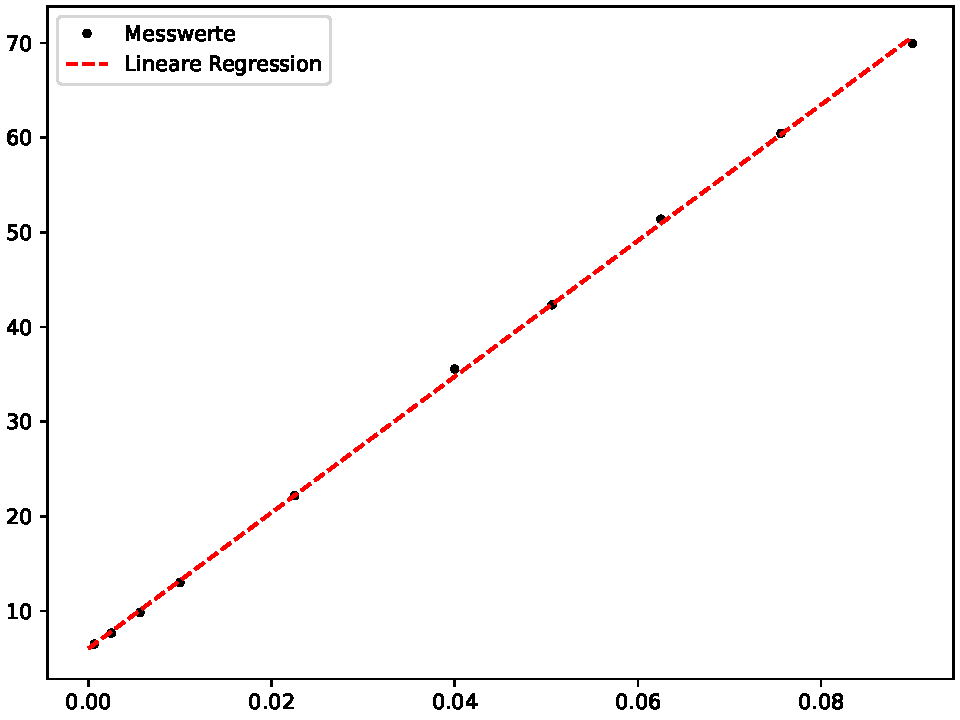
\includegraphics[width=\textwidth]{build/plot.pdf}
  \caption{Dargestellt ist die Temperatur beider Wasserbehälter abhängig von der Zeit. Die Zeit wurde in Sekunden umgerechnet und die Temperatur in Kelvin.}
  \label{fig:plot}
\end{figure}

\subsection{Differentialquotienten}
Die allgemeine Ableitung eines quadratischen Polynoms entspricht 
\begin{equation*}
  f=2a*t+b
\end{equation*}
.
Mit den Formeln \ref{eqn:gütemittel} und \ref{eqn:wärmemenge} ergibt sich die Formel
\begin{equation}
\nu=\frac{1}{N}(m_1c_{\symup{w}}+m_{\symup{k}}c_{\symup{k}})\frac{\increment T_1}{\increment t}
\label{eqn:nuu}
\end{equation}
, welche analog auch für $T_2$ gilt.
Für die Berechnung werden die Werte für die Differentialquotienten $\frac{\increment T_1}{\increment t}$ und $\frac{\increment T_2}{\increment t}$ für vier 
verschiedene Werte von t berechnet und in Tabelle \ref{tab:tabelle2} aufgeführt.
Die Fehler wurden mit der Formel
\begin{equation}
    \increment f=\sqrt{\sum_{i=1}^{\symup{n}} (\frac{\partial f}{\partial x_i})^2 (\increment x_i)^2}
\end{equation}
berechnet.

\begin{table}[H]
  \centering
  \caption{Hier sind die Werte für die Differentialquotienten von vier verschiedenen Werten von t aufgeführt.}
  \label{tab:tabelle2}
  \begin{tblr}{
    colspec={S[table-format=2.0] S[table-format=1.5] S[table-format=1.4] S[table-format=2.4] S[table-format=1.4]},
    row{1}={guard,mode=math},
    vline{3} = {2}{-}{text=\clap{$\pm$}},
    vline{5} = {2}{-}{text=\clap{$\pm$}},
  }
  \toprule
  t \mathbin{/} \unit{\minute} & \SetCell[c=2]{c} \frac{\symup{dT_1}}{\symup{dt}} \mathbin{/} \unit{\kelvin\per\second}& 
  & \SetCell[c=2]{c} \frac{\symup{dT_2}}{\symup{dt}}\mathbin{/} \unit{\kelvin\per\second}&\\
  \midrule
  4     &   0.02447  & 0.00035    &   0.0228    &   0.0004    \\
  8     &   0.0215   & 0.0004    &    0.0247    &   0.0004   \\
  12    &   0.0186   & 0.0005    &    0.0267    &   0.0005  \\
  16    &   0.0156   & 0.0005    &    0.0287    &   0.0006  \\
  \bottomrule
  \end{tblr}
\end{table}

Diese werden nun in Gleichung \ref{eqn:nuu} eingesetzt.
Mit der Masse des Wassers $m_1=\qty{3}{\kilo\gram}$, seiner spezifischen Wärmekapazität $c_{\symup{w}}=\qty{4200}{\joule\per\kilo\gram}$ (\cite{WasserWärme})
und der Wärmekapazität des Behälters und der Kupferschlange $m_{\symup{k}}c_{\symup{k}}=\qty{750}{\joule\per\kilo\gram}$ kann $\nu$ berechnet werden.
Damit ergeben sich die Werte in Tabelle \ref{tab:tabelle3}.
Zudem wird die idealisierte Gütezahl mit \ref{eqn:güteideal} bestimmt.
Die Abweichung zwischen rellem und idealen Wert wird mit 
\begin{equation}
  |A_{i,r}|=\frac{\nu_{\symup{ideal}}-\nu_{\symup{real}}}{\nu_{\symup{ideal}}}
  \label{eqn:Abweichung}
\end{equation}
berechnet.

 \begin{table}[H]
   \centering
   \caption{Aufgelistet sind der experimentell bestimmte Wert für die Güteziffer, sowie der berechnete Wert für die einer idealen Wärmepumpe und die dazugehörige Abweichung.}
   \label{tab:tabelle3}
   \begin{tblr}{
     colspec={S[table-format=2.0] S[table-format=1.2] S[table-format=1.2] S[table-format=2.3] S[table-format=1.3] S[table-format=2.2] S[table-format=1.2]},
     row{1}={guard,mode=math},
     vline{3} = {2}{-}{text=\clap{$\pm$}},
     vline{5} = {2}{-}{text=\clap{$\pm$}},
     vline{7} = {2}{-}{text=\clap{$\pm$}},
   }
   \toprule
   t \mathbin{/} \unit{\minute} &\SetCell[c=2]{c} \nu_{\symup{real}}  && \SetCell[c=2]{c}  \nu_{\symup{ideal}} && \SetCell[c=2]{c} A \mathbin{/} \unit{\percent}&\\
   \midrule
   4     &   2.72   &   0.04    &    31.500    &   0.500    &      91.36    &   0.18     \\      %2.53     &     0.04 &       \\
   8     &   2.39   &   0.04    &    15.710    &   0.110    &      84.79    &   0.28     \\      %2.75     &     0.05 &       \\
   12    &   1.98   &   0.05    &    11.020    &   0.050    &      82.00    &   0.50     \\      %2.85     &     0.06 &       \\
   16    &   1.81   &   0.06    &     8.835    &   0.033    &      79.50    &   0.70     \\      %3.33     &     0.07 &       \\
   \bottomrule 
   \end{tblr}
 \end{table}

 \subsection{Berechnung des Massendurchsatzes}

Zur Bestimmung des Massendurchsatzes wird die Gleichung \ref{eqn:masse} verwendet. Die Summe der Wärmekapazitäten lässt sich hier 
direkt als $m_2c_{\symup{w}}+m_{\symup{k}}c_{\symup{k}}=\qty{13150}{joule\per\kelvin}$ bestimmen. Dazu muss noch die Verdampfungswärme
$L$ bestimmt werden.

\begin{figure}
    \centering
    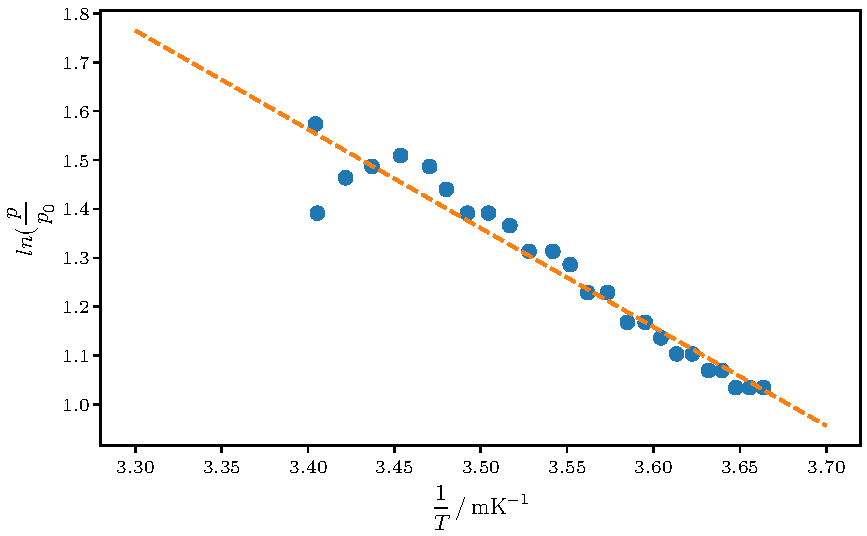
\includegraphics{verdampfplot.pdf}
    \caption{Der Druck bei dem kalten Reservoir gegen dessen Temparatur.}
    \label{fig:druckkalt}
\end{figure}

Mithilfe einer linearen Regression, die aussieht wie $ln(\frac{p}{p_0})=a\frac{1}{T_2}+b$ und der Gleichung \ref{eqn:verdampf},
lässt sich hier feststellen, dass die Verdampfungswärme $L=-a \cdot R$ einen Wert von $\qty{243(14)}{\joule\per\mole}$ annimmt.
Hierbei beträgt der Umgebungsdruck $p_0=\qty{0.9949}{\bar}$. \cite{pDortmund}

Mit der den Gleichungen \ref{eqn:gütemittel} und \ref{eqn:Dampf} ergitbt sich 
\begin{equation*}
  \frac{\increment m}{\increment t}=\frac{\nu N}{L}
\end{equation*}
kann dann der Massendurchsatz berechnet werden.
Damit ergibt sich ein Wert für $L=\qty{}{}$


\begin{table}[H]
  \centering
  \caption{Dargestellt sind die Werte für den Massendurchsatz für verchiedene Zeiten.}
  \label{tab:tabelle4}
  \begin{tblr}{
    colspec={S[table-format=2.0] S[table-format=2.1] S[table-format=1.1]},
    row{1}={guard,mode=math},
    vline{3} = {2}{-}{text=\clap{$\pm$}},
  }
  \toprule
  t \mathbin{/} \unit{\minute} &\SetCell[c=2]{c} \frac{\increment m}{\increment t} \mathbin{/} \unit{\joule\per\kilo\gram} &\\
  \midrule
  4     &   78.0   &   5.0     \\
  8     &   68.0   &   4.0    \\
  12    &   57.0   &   4.0    \\
  16    &   51.7   &   3.4     \\
  \bottomrule 
  \end{tblr}
\end{table}